\chapter{Implementation}
\section{Implementation Details and Encountered Challenges}
\subsection{Beat Logic}
Since the game relies heavily on fixed beats that correspond to the music, we decided to create a central metronome object. The metronome ended up supporting two ways of identifying the current beat, a beatID property returning the current beat, and a callback called on each beat update. All game objects were originally intended to register as listeners to the ''OnBeatTickCallback''. However, as we were not in total control over the order of callback executions, we ran into logical inconsistencies in the cueing system. We worked around this issue by only registering callbacks in order independent systems. During these callbacks, each system would be responsible for updating their order dependent subsystems through direct function calls. This introduces some more coupling into the codebase, but not to an unmanageable degree. 

\subsection{Audio Playback}
Requiring the player to cue in different instruments throughout a song, un-muting individual instruments on success or muting them on failure, presented an interesting challenge. Controlling the different tracks was done through a simple enum, however, we ran into issues that the tracks were not necessarily synchronized, which was devastating to the game. Luckily Unity’s AudioSource supports scheduling tracks, fixing the synchronization problem~\cite{unity_audio_source_api}. 

\subsection{Cues}
\begin{figure}[tbph]
    \centering
    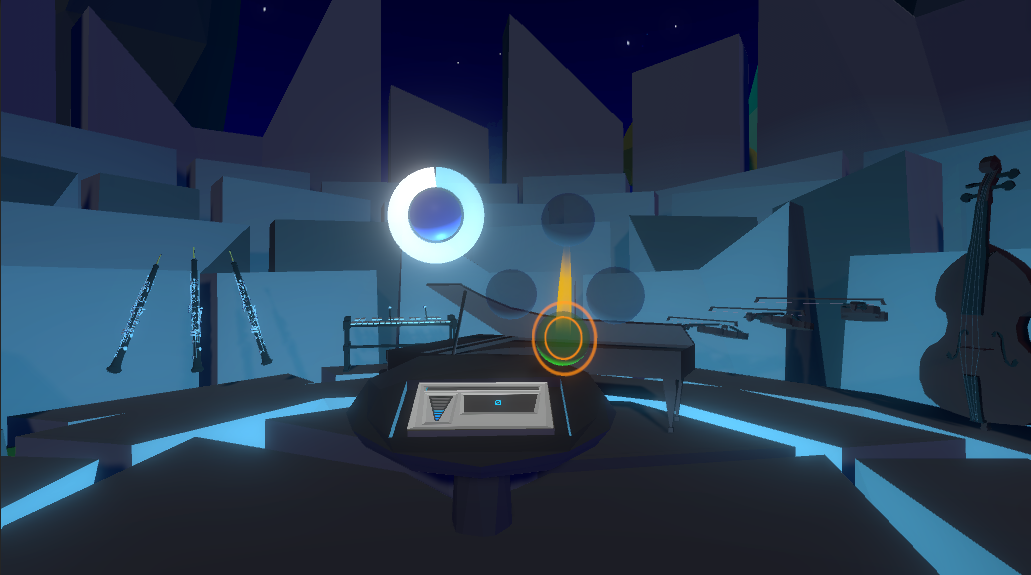
\includegraphics[width=1.0\textwidth]{images/cue}
    \caption[Screenshot of a Cue]{This screenshot shows a Cue that is ready to be hit by the player to signify that an instrument track should start playing.}
    \label{fig:cue}
\end{figure}

The musical cues were implemented as a finite state machine as seen in Figure~\ref{fig:cue_fsm}. The cue transitions between different states are based on the number of beats left before the instrument should enter and whether or not it has been hit by the player. Implementing the cues as a finite state machine allowed us to structure the code in a way that was consistent with the state transitions of the cue, making it easy to follow the logical execution of the cue behavior. 
An alternative solution could be to go with a full state pattern\cite{game_programming_patterns}, with separate classes for each state. However, we did not deem the cue logic to be complex enough to justify such a solution. An example of a cue can be seen in Figure~\ref{fig:cue}.

\begin{figure}[tbph]
    \centering
    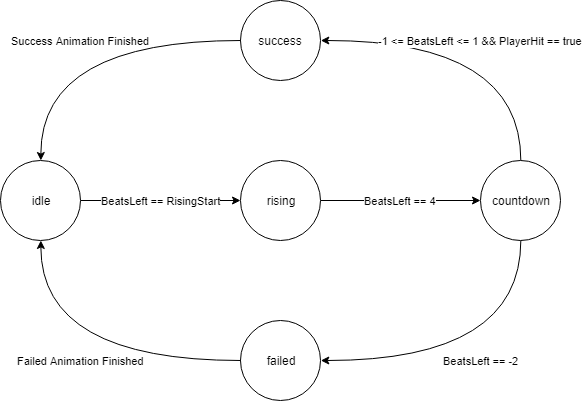
\includegraphics[width=1.0\textwidth]{images/cue_fsm}
    \caption[Cue Finite State Machine]{This model shows the finite state machine used for the cueing logic}
    \label{fig:cue_fsm}
\end{figure}

\subsection{Creating an illusion of glowing light for objects without light sources}
In terms of the in-game environment, the original plan was to include bright glowing mushrooms scattered around the area. A problem arose when the number of illuminated mushrooms in the scene exceeded a manageable amount, severely reducing the performance of the application. We wanted to keep the visual integrity of the scene as close as possible to its original Blender model, so we came up a workaround for the problem.

Instead of illuminating the mushrooms, we worked around the issue by changing their material to a bright colour. We then added a bloom post-processing effect, creating an illusion of glowing light around the mushrooms. This did not light up the scene in any way, but the small size of the mushrooms and the sheer amount of them made this the most logical solution to keep the visuals intact without sacrificing performance. 

\subsection{Creating simple fog effects using Unity's particle system}
\begin{figure}[tbph]
    \centering
    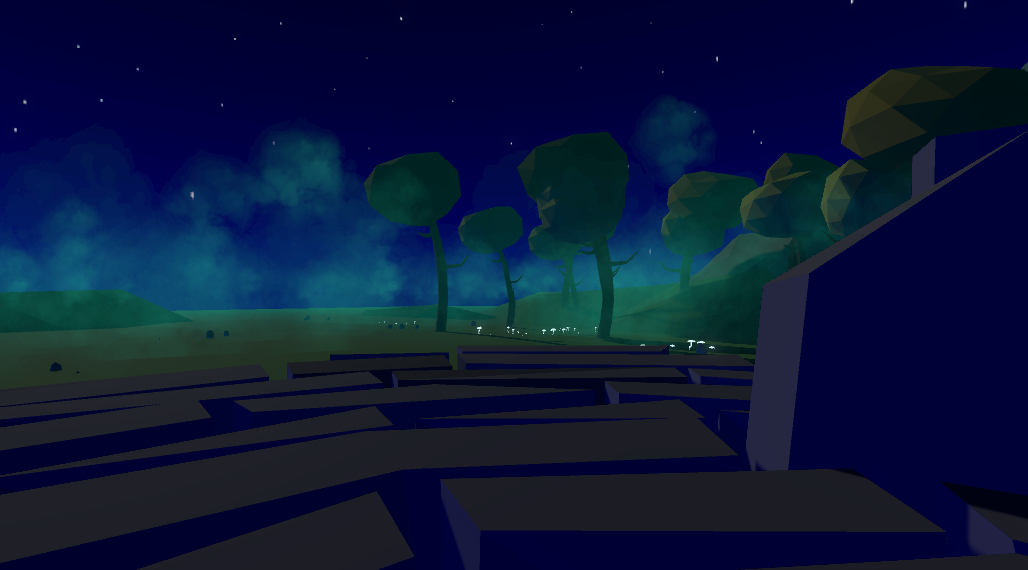
\includegraphics[width=1.0\textwidth]{images/fog}
    \caption[Screenshot of ingame fog]{This screenshot showcases how the ingame fog looks like.}
    \label{fig:fog}
\end{figure}
The original concept idea for the in-game environment also included some green fog that was spread around in the scene. Ideally, this could be handled through the use of Volumetric Fog or similar implementations, but due to limited time to work on the project, we had to find a quicker and simpler solution to implement while still providing a relatively good approximation of the fog effect. 

We implemented fog using Unity's Particle System component, utilizing a single fog texture from the Unity particle effects standard assets pack. We then layered several particle systems on top of each other with small variations in settings like particle size, rotation, lifetime, and, emission rate to create the illusion of fog. We combined this with Unity’s distance fog functionality which makes geometry fade towards a gradient colour based on distance from the camera. This enhances the illusion of fog. The end result does not look equivalent to Volumetric Fog, but we believe it serves its purpose, and saved us a good amount of development resources. A screenshot illustrating the visuals of the fog can be seen in Figure~\ref{fig:fog}. 


\subsection{Demonstrating the conducting pattern visually}
\begin{figure}[tbph]
    \centering
    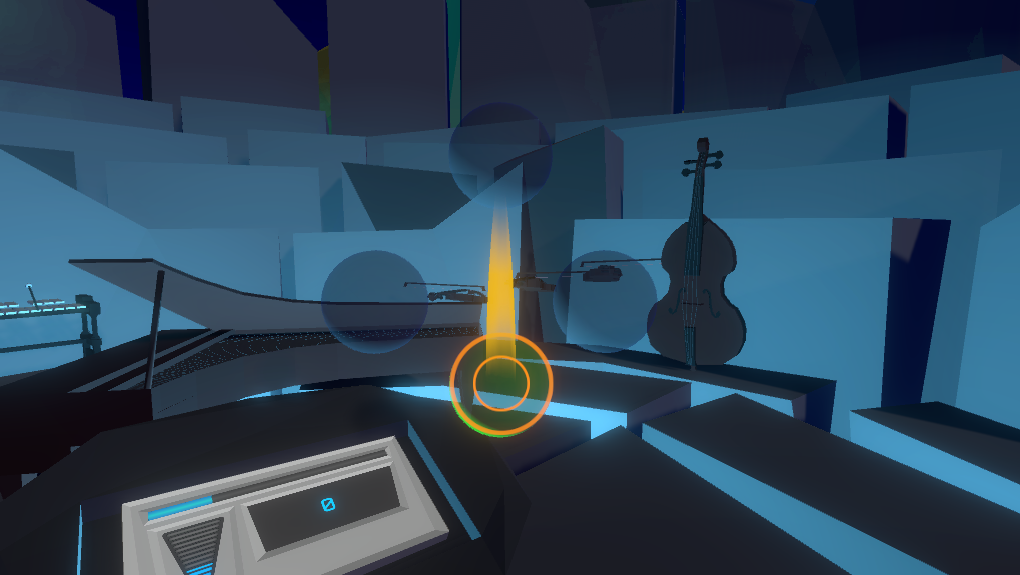
\includegraphics[width=1.0\textwidth]{images/spheres-trail-pulse}
    \caption[Screenshot of Motion Tracking Spheres]{This screenshot illustrates the four motion tracking spheres used for conducting. The currently active sphere is coloured green with expanding circles emmitting at the start of the beat. There is also a trail that further illustrates how the player should move their hand between beats.}
    \label{fig:trackingspheres}
\end{figure}
The initial implementation for demonstrating the conducting pattern included four transparent spheres. These spheres would change their material from a gray to a green colour, indicating that the player was supposed to touch it at that beat. This method made it possible to see the conducting pattern as only one sphere would be green at any given time, and the colour changed on beat which reinforced the rhythmic movement to the player. While the initial implementation was fine for internal testing, later playtesting with externals provided some insight into the fact that more visual feedback and information would be preferred. This was particularly apparent for testers with no prior experience in conducting as they did not understand how they were supposed to move their hands. 

Our solution to this was to create trails between the four different spheres which demonstrated the pattern in a slightly more visual manner. 
This was handled by taking an invisible ''GameObject'' with a ''TrailRenderer'' and interpolate it between the previous beat's sphere and the next beat’s sphere.

To emphasize the rhythm we added expanding circles instantiated on the beat. These also indicated the next step in the conducting pattern. Additionally, the first beat was emphasized with a different colour to more easily allow the player to get back into the rhythm. This can be seen in Figure~\ref{fig:trackingspheres}. 

If more time was available, we would probably have used Bezier curves to demonstrate the conducting pattern in a more correct manner rather than having linear trails between the spheres. The added complexity of this approach is negligible, but it would take a fair amount of time to create proper looking curves without any visual aids in the Unity editor for bezier curve control. 


\subsection{Binding animation states to the beat}
To emphasize the rhythm of the song in Conductor Hero we ended up tying the majority of animation states to the ''OnBeatTickCallback'' in the Metronome component. While this was an interesting way to work with animations it also posed a fair share of problems. An issue with changing animation states on beat was the cases where it would be preferable to change the animation at different times than the callback. An example of this issue is detailed below: 

The player is supposed to start moving their hand towards the next beat before it starts, but the interpolated trail only starts moving towards the next sphere whenever the next beat triggers the beat callback. With a linear interpolation, this means that the trail lags behind where the player should have moved their hand between two beats, potentially confusing the player and making it hard to read the rhythm from the movement of the trail. To work around this we slightly modified the linear interpolation by parameterizing the input time through the use of an ''AnimationCurve''. This makes it possible to control the velocity of the animation throughout its lifetime. Using this, we made the velocity of the trail very fast early on, to create a more natural motion towards its destination to where the player needs to move their hand. 


\subsection{Providing Visual Player Feedback}
\begin{figure}[tbph]
    \centering
    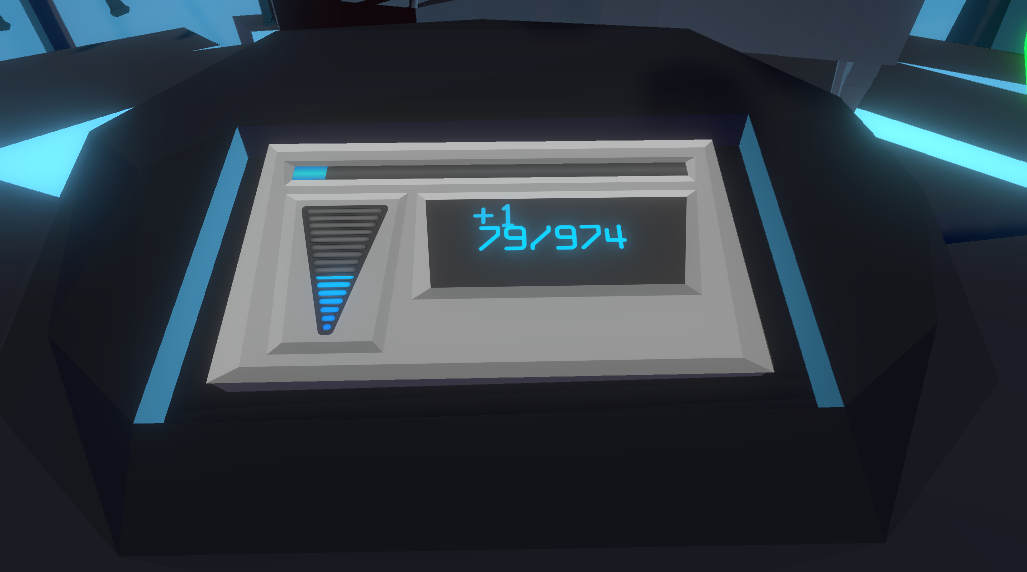
\includegraphics[width=1.0\textwidth]{images/scorePopup}
    \caption[Screenshot of the Conductor Table Dashboard]{This screenshot shows the dashboard on the Conductor Table where the top bar is current song progress, the left bar is the volume bar and the display on the right shows current score compared to maximum score.}
    \label{fig:table}
\end{figure}

It is important to provide the player with enough visual feedback for them to understand how their actions are being reflected in the game. In Conductor Hero, visual feedback is provided using several methods. 

Particle effects in the tracking spheres indicate whether or not the player is conducting correctly. Red particles indicate that the player is off beat, while green signifies being on beat.

We are also providing some visual feedback on the conductor table whenever the player gains score for either conducting on beat or hitting cues. 

A small popup appears in the table’s canvas whenever the score is increased, telling the player how much score their actions have resulted in. A score of ''+10'' is given for hitting cues correctly while a score of ''+1'' is given for every conducting motion that is on beat. The score values obtained by hitting cues could have been bigger, and more visually distinct, to further emphasize the larger amount of points gained, but we did not implement this due to time constraints. The visual feedback used in the conductor table can be seen in Figure~\ref{fig:table}.

\subsection{Design of the in-game environment}
\begin{figure}[tbph]
    \centering
    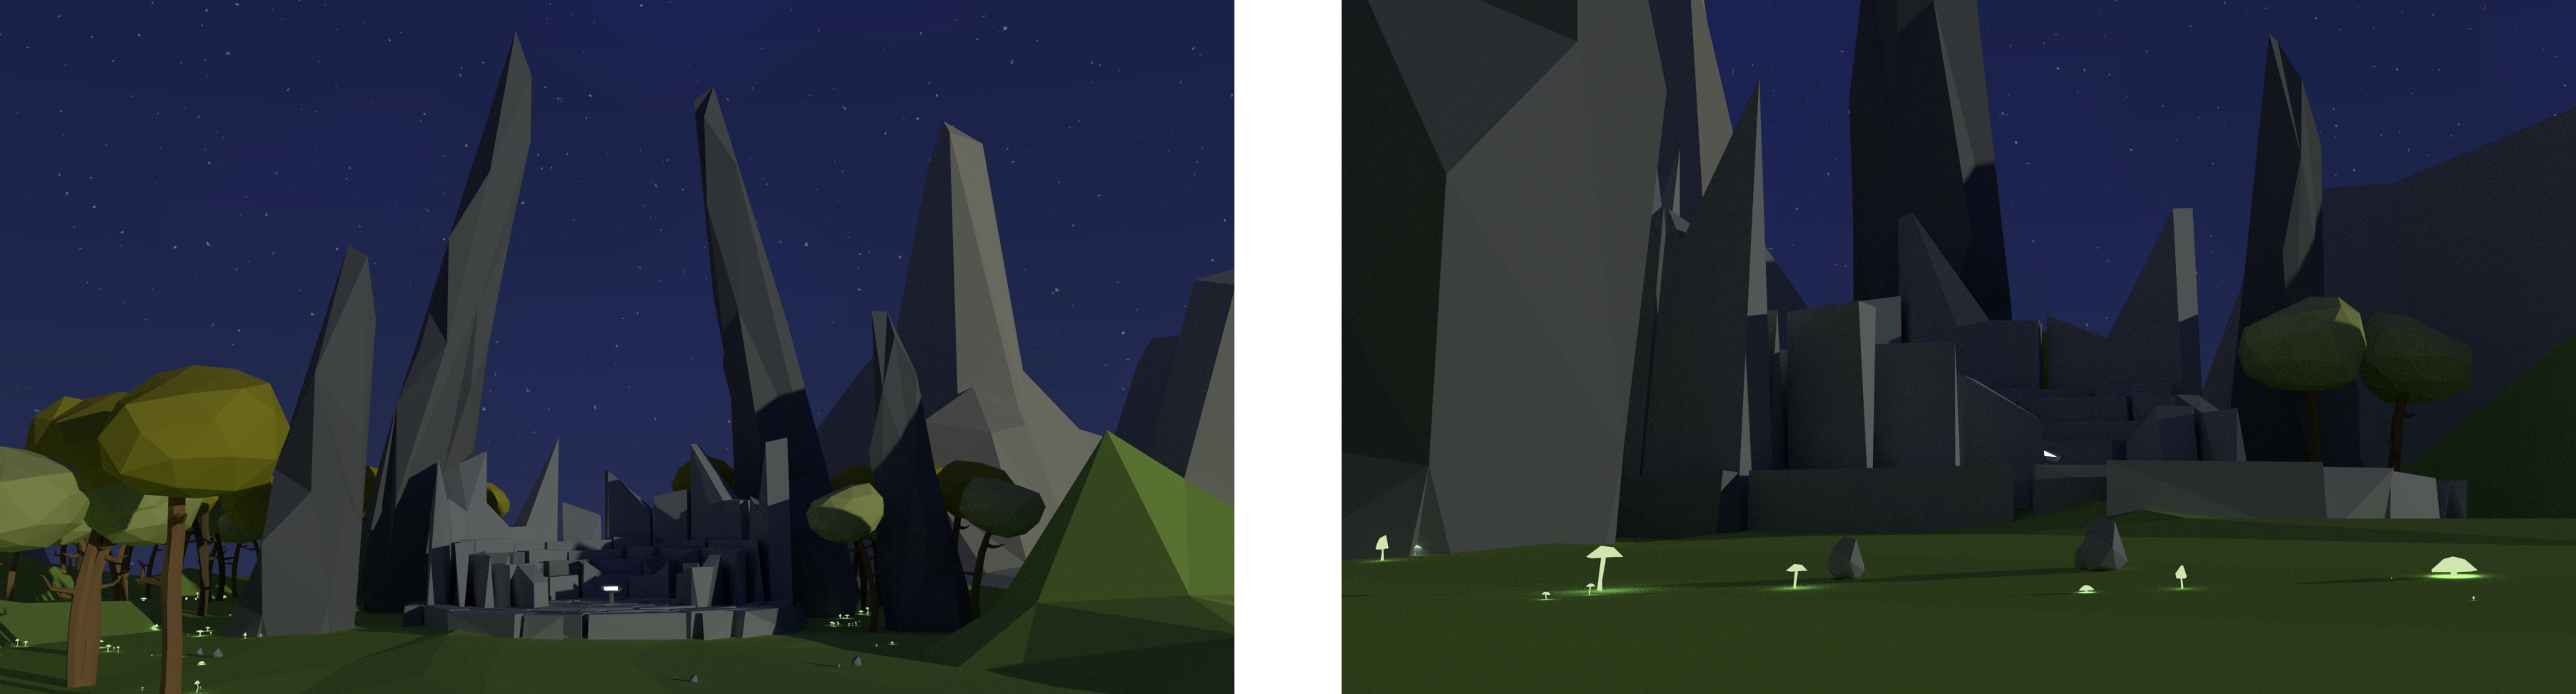
\includegraphics[width=1.0\textwidth]{images/Forest}
    \caption[The forest scene from the prototype]{These screenshots showcase the 3D environment made in Blender.}
    \label{fig:Forest}
\end{figure}

\begin{figure}[tbph]
    \centering
    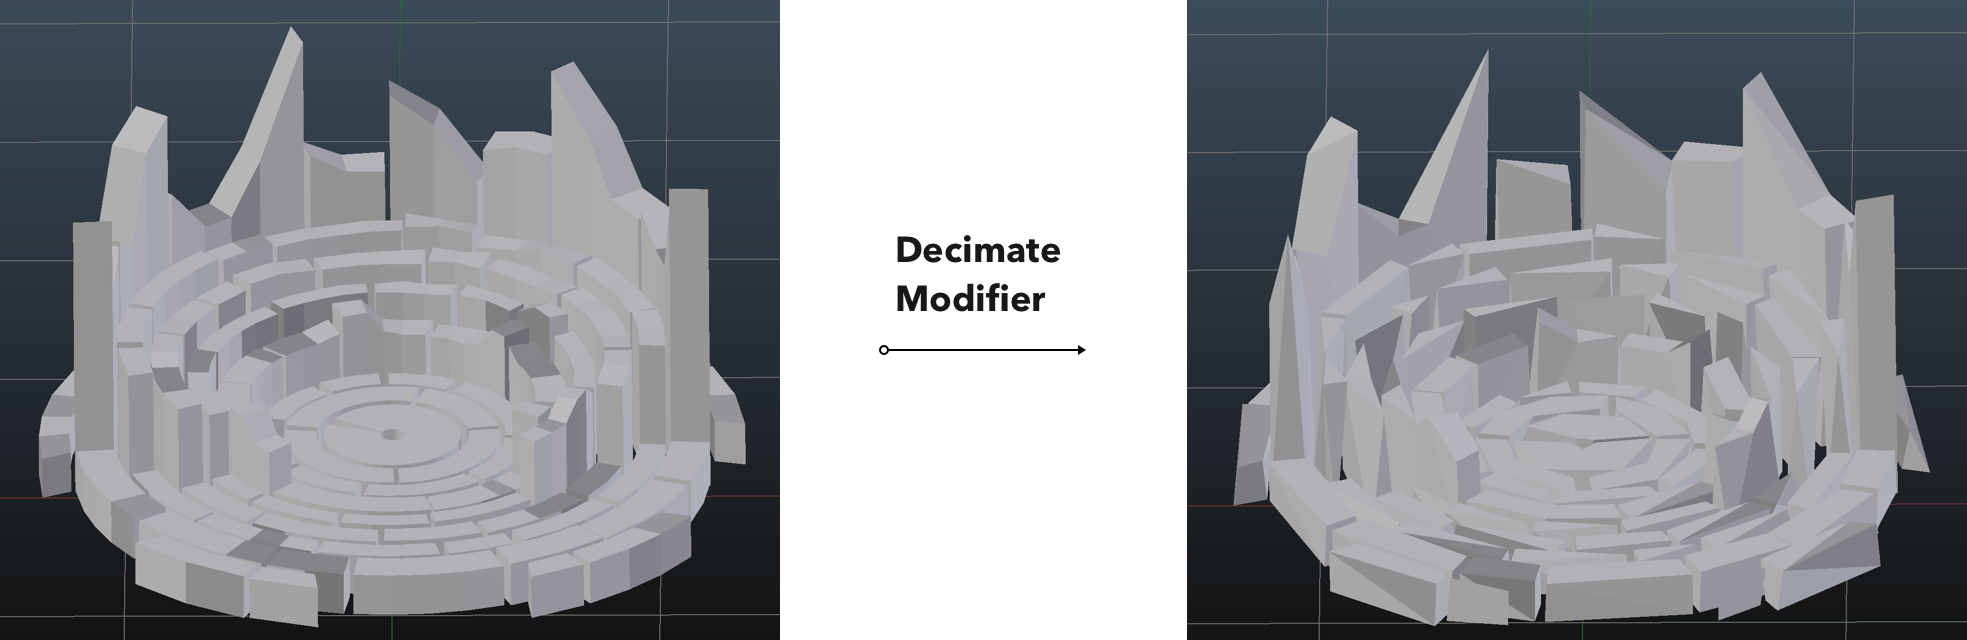
\includegraphics[width=1.0\textwidth]{images/lowPolyDecimate}
    \caption[Example use of the Decimate Modifier in Blender]{This figure illustrates how the Decimate Modifier in Blender can create a low poly version of a regular 3D model.}
    \label{fig:lowpolydecimate}
\end{figure}


A goal of Conductor Hero was to immerse the players into a unique VR environment while conducting the orchestra. We discussed various environments like a seabed, or the outer space, but settled on the forest scene for the prototype due to time constraints. We envisioned that the musicians of the orchestra could change to fit the environment, turning into beasts, fish, or aliens. The game has a low poly style, as the concept did not require high-fidelity graphics. We believe that the visuals look appealing to the audiences while being stylish, they are easy to create and iterate upon, which has the added benefit of fitting within the time scope of our project. To achieve this style we used the Decimate modifier in Blender to decrease the number of polygons in each object. An example of how the modifier was used can be seen in Figure~\ref{fig:lowpolydecimate} while the final 3D model of the environment can be seen in Figure~\ref{fig:Forest}. We reviewed existing games using low poly styles and imagery of forests to create a harmonious colour palette for our scene. The colour palette we ended up using is shown in Figure~\ref{fig:colourpalette}. During this review, we found that many existing rhythm games use lighting to emphasize the rhythmic feel of the song. To achieve the same effect we introduced lighting into the floor that the player is standing on, which pulsates with the rhythm. The cyan light below the stage and the ''glowing'' mushrooms around the environment further enhance the fantasy theme of the scene.

\begin{figure}[H]
\centering
    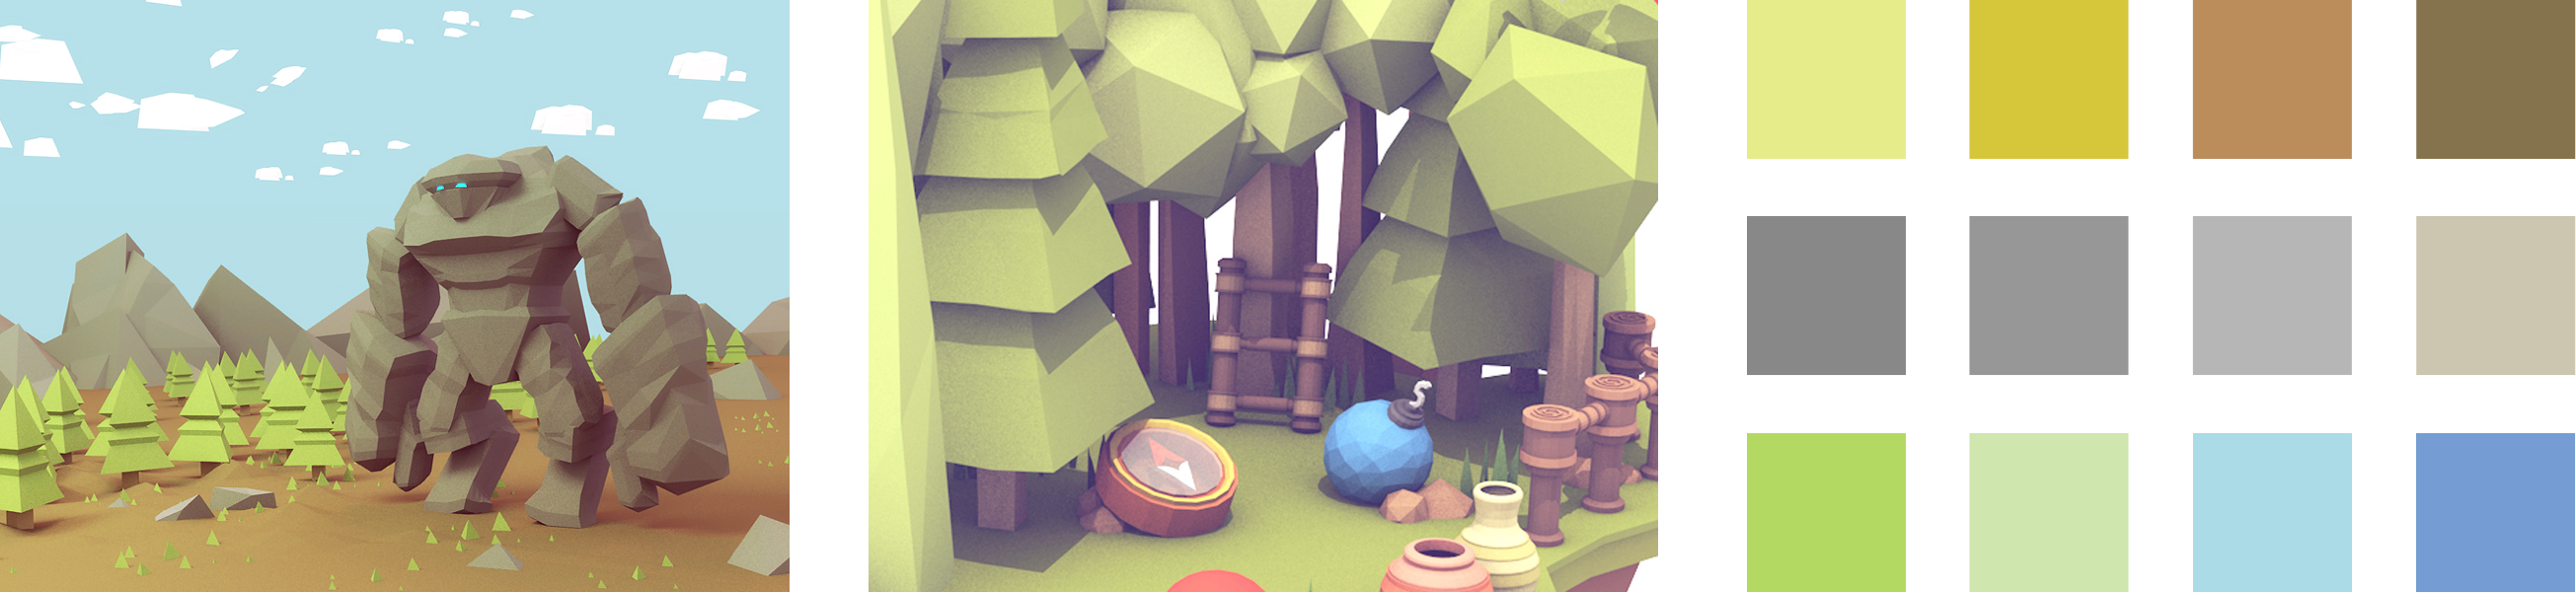
\includegraphics[width=1.0\textwidth]{images/sceneColourPalette}
    \caption[The colour palette for the ingame scene]{The colour palette we used in the project was influenced by styles similarly to what is illustrated here. The final colour palette is seen on the right. }
    \label{fig:colourpalette}
\end{figure}